\newcommand{\DiagramScale}{0.6}
\chapter{PCLc}
PLCc is the PCL compiler. It is located in the \texttt{src/pclc} directory of the Git clone and your path should be set according. This chapter introduces the PCL syntax using \emph{railroad diagrams}. Railroad diagrams illustrate valid PCL and are read from left to right, following the lines as a train would. The symbols in the yellow ovals are to be typed \emph{as is}. The symbols in the tan rectangles references another railroad diagram. The referenced diagram should be used to expand the rectangle in more valid PCL. Hexagons contain \emph{character classes} and specify a range of characters that will be accepted.

\section{PCL Syntax}
\begin{figure}[h!]
  \centering
    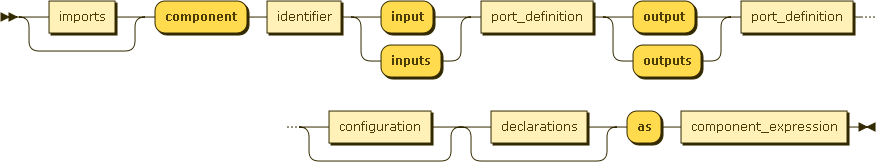
\includegraphics[scale=\DiagramScale,angle=90]{chapters/compiler/diagrams/component}
  \caption{PCL file syntax.}
  \label{fig:pcl-top-level}
\end{figure}
The top level symtax of a PCL file is shown in Figure \ref{fig:pcl-top-level}, and consists of the following sections:
\begin{itemize}
\item \textbf{Imports}: Imports can be optionally specified. Importing, as in other language, makes available other components to the PCL component being written.
\item \textbf{Component}: This starts the component definition and provides the name. The component's name must be the same as the filename. E.g., a component in \texttt{fred.pcl} must be called \texttt{fred}.
\item \textbf{Inputs}: Defines the inputs of the component. This information is used to verify that the outputs of a previous component is compatible with another.
\item \textbf{Outputs}: Defines the outputs of the component. This information is used to verify that the inputs of a subsequent component is compatible with another.
\item \textbf{Configuration}: Optional configuration for the component. This is static data that shall be used to construct imported components used in this component. 
\item \textbf{Declarations}: Optional declarations of components used in this component. This is where the import components are constructed.
\item \textbf{Definition}: This portion is the component definition. It is an expression which defines how the constructed components are to be combined to create the computation required.
\end{itemize}

\subsection{Imports}\label{subsec:imports}
\begin{figure}[h!]
  \centering
    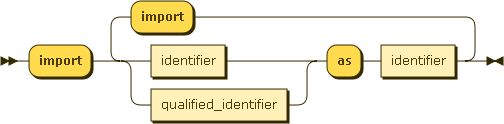
\includegraphics[scale=\DiagramScale]{chapters/compiler/diagrams/imports}
  \caption{\texttt{imports} : Importing PCL files.}
  \label{fig:pcl-imports}
\end{figure}
Extant PCL components can be used in other PCL components. The mechanism for using components is through importing. There can be zero or more imports in a PCL file. Figure \ref{fig:pcl-imports} shows the syntax for importing.

The imported component is referenced using an identifier which can be fully qualified using a dot separated name. If the component is referenced using one or more dots the sequence of idenitifiers, apart from the last one, is used to address a package of components. The last identifier specifies the component name. The environment variable \texttt{PCL\_IMPORT\_PATH} is a colon separated list of directories from which a search shall take place for the PCL components. If this enivronment variable is not set then the current working directory is used as a starting point for the component search.

Each imported component must specify an alias. This is the name by which this component shall be refered to in this PCL file. E.g., \texttt{import components.utility.sleep as sleep\_comp} shall import a PCL component called \texttt{sleep} from the package \texttt{components.utility} and shall be refered to as, i.e. has the alias, \texttt{sleep\_comp}.

\subsection{Port Definition}
\begin{figure}[h!]
  \centering
    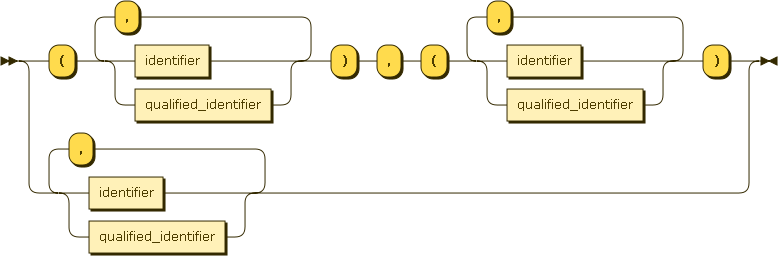
\includegraphics[scale=\DiagramScale,angle=90]{chapters/compiler/diagrams/port_definition}
  \caption{\texttt{port\_definition} : Component port definition.}
  \label{fig:pcl-port-def}
\end{figure}
A port definition informs the PCL compiler about the nature of a component's input or an output. Components can have 2, 3 or 4 ports: one input and output port, one input port and two output ports, two input ports and one output port, or two input and output ports. Figure \ref{fig:pcl-port-def} shows the syntax for this grammatical construct.

A port can carry one or more \emph{signals}. A signal is a piece of data that flows through ports and has a unique name to that port, and can be fully qualified\footnote{It may be easier to group signals through the use of a hierarchical naming convention, e.g., \texttt{a.b.c} and \texttt{a.b.d}.}. The signal names, for a port, are declared in a port definition. The ``shape'' of a port definition declares whether an input or an output has one or two ports. For example, consider the following input and output port definitions:
\begin{itemize}
\item A component with one input and one output port. Input signals are \texttt{tom}, \texttt{dick}, \texttt{harry} and output signals are \texttt{disley} and \texttt{standedge}.
\begin{center}
\begin{verbatim}
component tunnel
    inputs tom, dick, harry
    outputs disley, standedge
    ...
\end{verbatim}
\end{center}

\item A component with one input and two output ports. Input signal is \texttt{fruit.banana}. The \emph{top} output port signal is \texttt{veg.carrot} and the \emph{bottom} output port signals are \texttt{fruit.super}, and \texttt{fruit.salad}.
\begin{center}
\begin{verbatim}
component split
    inputs fruit.banana
    outputs ( veg.carrot ), ( fruit.super, fruit.salad )
    ...
\end{verbatim}
\end{center}

\item A component with two inputs and one output port. Input signals for the \emph{top} port are \texttt{tea} and \texttt{coffee}, and the signals for the \emph{bottom} port are \texttt{milk}, and \texttt{water}. The output port's single signal is \texttt{drink}.
\begin{center}
\begin{verbatim}
component pot
    inputs ( tea, coffee ), ( milk, water )
    outputs drink
    ...
\end{verbatim}
\end{center}

\item A component with two input and output ports. Input signals for the \emph{top} port are \texttt{zippy} and \texttt{george}, and the signals for the \emph{bottom} port are \texttt{rod}, \texttt{jane}, and \texttt{freddy}. The output signals are for the \emph{top} port are \texttt{geoffrey}, and the \emph{bottom} port signals are \texttt{bungle} and \texttt{zippo}.
\begin{center}
\begin{verbatim}
component rainbow
    inputs ( zippy, george ), ( rod, jane, freddy )
    outputs ( geoffrey ), ( bungle, zippo )
    ...
\end{verbatim}
\end{center}

\end {itemize}

\subsection{Configuration}
\begin{figure}[h!]
  \centering
    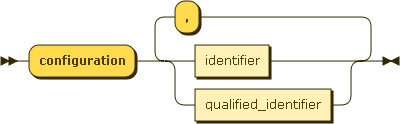
\includegraphics[scale=\DiagramScale]{chapters/compiler/diagrams/configuration}
  \caption{\texttt{configuration} : Component configuraton.}
  \label{fig:pcl-config}
\end{figure}
A component's configuration is static data that is primarily used for constructing import components. Configuration data is named using identifiers, which can be fully qualified. Figure \ref{fig:pcl-config} shows the configuration syntax. Configuration identifiers may also be used in \emph{if} components see Section \ref{sec:cond-expr} for details. A PCL can declare zero or more configuration identifiers.

Figure \ref{fig:pcl-config-example} shows an example of configuration being declared in a PCL file. Here the \texttt{parallel\_sleep} component shall be constructed using two configuration values, namely \texttt{sleep\_command} and \texttt{sleep\_time}.
\begin{figure}[h!]
\begin{center}
\begin{verbatim}
import sleep as sleep

component parallel_sleep
    ...
    configuration sleep_command, sleep_time
    ...
\end{verbatim}
\end{center}
\caption{Example declaration of PCL configuration.}
\label{fig:pcl-config-example}
\end{figure}

\subsection{Declarations}
\begin{figure}[h!]
  \centering
    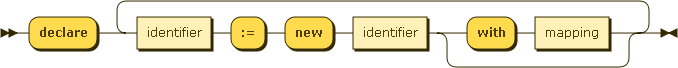
\includegraphics[scale=\DiagramScale]{chapters/compiler/diagrams/declarations}
  \caption{\texttt{declarations} : Imported component construction.}
  \label{fig:pcl-decls}
\end{figure}
The declaration section of a PCL file is where the imported components can be constructed using the configuration available in the importing component's PCL. Figure \ref{fig:pcl-decls} shows the syntax for component construction. All declarations are assigned to an identifier which shall be unique. The import alias (see Section \ref{subsec:imports}) is used to reference the imported component from which an instance is created. There is an optional \emph{with} clause which allows configuration to be mapped into a component's constructor. Figure \ref{fig:pcl-decl-example} shows a PCL snippet that is an example of constructing imported components. Here two instances of the same component are constructed, namely the \texttt{sleep} component, which has the alias \texttt{sleep\_component}. The \texttt{sleep} component specifies the configuration \texttt{command.sleep} so the \emph{with} clause maps the \texttt{parallel\_sleep} component's configuration to the \texttt{sleep} component's configuration.
\begin{figure}
\begin{center}
\begin{verbatim}
import sleep as sleep_component

component parallel_sleep
    input sleep_time
    outputs (complete), (complete)
    configuration sleep_command
    declare
        top_sleep := new sleep_component
            with sleep_command -> command.sleep
        bottom_sleep := new sleep_component
            with sleep_command -> command.sleep
    ...
\end{verbatim}
\end{center}
\caption{Example of component construction.}
\label{fig:pcl-decl-example}
\end{figure}


\subsection{Definition}
\begin{figure}[h!]
  \centering
    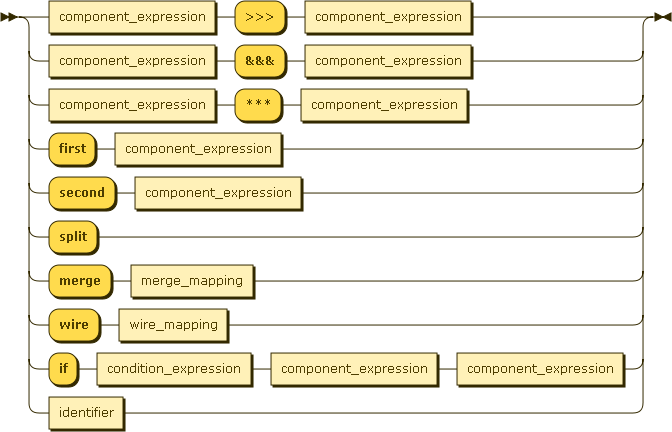
\includegraphics[scale=\DiagramScale,angle=90]{chapters/compiler/diagrams/component_expression}
  \caption{\texttt{component\_expression} : Component defintion.}
  \label{fig:pcl-def}
\end{figure}

\subsection{Merge Mapping}
\begin{figure}[h!]
  \centering
    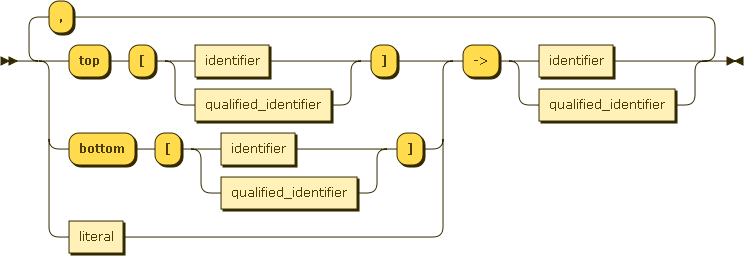
\includegraphics[scale=\DiagramScale,angle=90]{chapters/compiler/diagrams/merge_mapping}
  \caption{\texttt{merge\_mapping} : Merge component mapping.}
  \label{fig:pcl-merge-mapping}
\end{figure}

\subsection{Mapping}
\begin{figure}[h!]
  \centering
    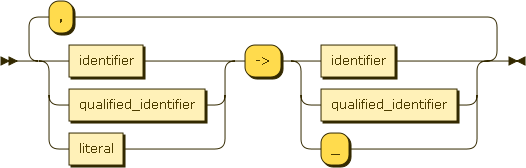
\includegraphics[scale=\DiagramScale]{chapters/compiler/diagrams/mapping}
  \caption{\texttt{mapping} : Mapping.}
  \label{fig:pcl-mapping}
\end{figure}

\subsection{Wire Mapping}
\begin{figure}[h!]
  \centering
    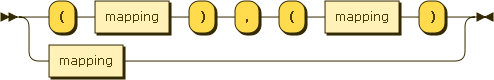
\includegraphics[scale=\DiagramScale]{chapters/compiler/diagrams/wire_mapping}
  \caption{\texttt{wire\_mapping} : Wire mapping.}
  \label{fig:pcl-wire-mapping}
\end{figure}

\subsection{Condition Expression}\label{sec:cond-expr}
\begin{figure}[!h]
  \centering
    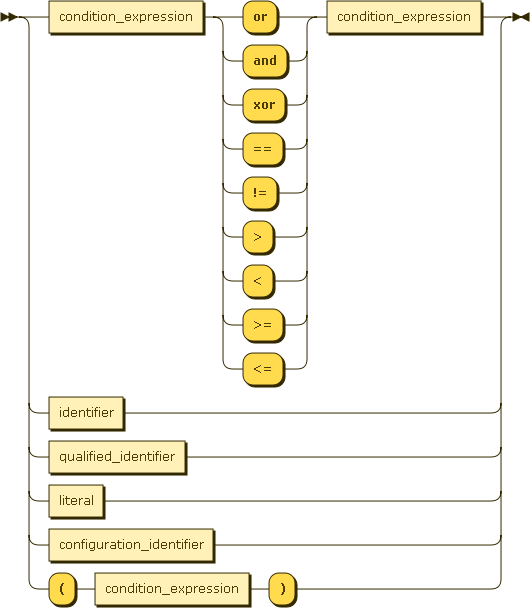
\includegraphics[scale=\DiagramScale]{chapters/compiler/diagrams/condition_expression}
  \caption{\texttt{condition\_expression} : If component's condition expression.}
  \label{fig:pcl-cond-expr}
\end{figure}

\subsection{Configuration Identifier}
\begin{figure}[!h]
  \centering
    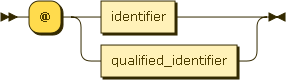
\includegraphics[scale=\DiagramScale]{chapters/compiler/diagrams/configuration_identifier}
  \caption{\texttt{configuration\_identifier} : If component's condition expression configuration identifier.}
  \label{fig:pcl-config-id}
\end{figure}

\subsection{Qualified Identifier}
\begin{figure}[!h]
  \centering
    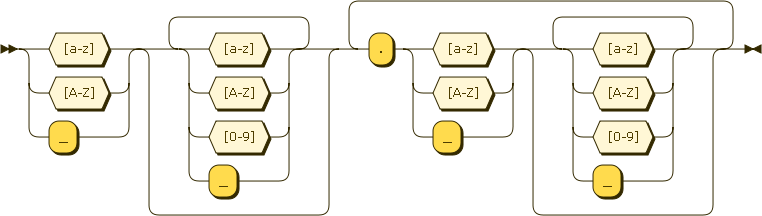
\includegraphics[scale=\DiagramScale,angle=90]{chapters/compiler/diagrams/qualified_identifier}
  \caption{\texttt{qualified\_identifier} : Qualified identifier.}
  \label{fig:pcl-qualified-id}
\end{figure}

\subsection{Identifier}
\begin{figure}[!h]
  \centering
    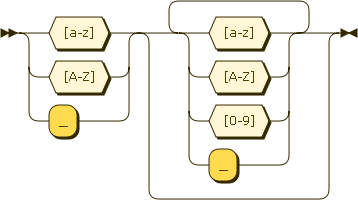
\includegraphics[scale=\DiagramScale]{chapters/compiler/diagrams/identifier}
  \caption{\texttt{identifier} : Identifier.}
  \label{fig:pcl-id}
\end{figure}

\subsection{Literal}
\begin{figure}[!h]
  \centering
    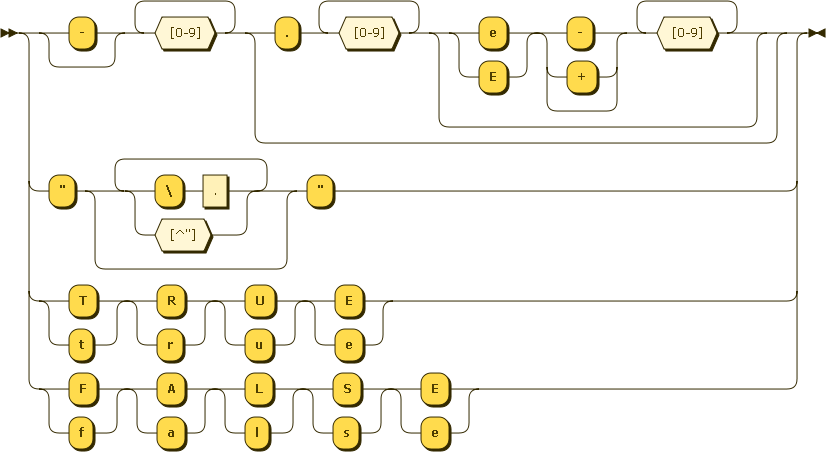
\includegraphics[scale=\DiagramScale,angle=90]{chapters/compiler/diagrams/literal}
  \caption{\texttt{literal} : Literal.}
  \label{fig:pcl-literal}
\end{figure}

\subsection{Example PCL file}
This example PCL file can be found in the \texttt{parallel\_sleep} example PCL.
\begin{figure}[!h]
  \begin{verbatim}
import sleep as sleep

component parallel_sleep
  input sleep_time
  outputs (complete), (complete)
  configuration sleep_command
  declare
    top_sleep := new sleep with sleep_command -> sleep_command
    bottom_sleep := new sleep with sleep_command -> sleep_command
  as
    top_sleep &&& bottom_sleep
  \end{verbatim}
  \caption{Example PCL file.}
\end{figure}

\section{Usage}
